\documentclass[UTF8,aspectratio=169]{ctexbeamer}
\usetheme{Madrid}
\usecolortheme{whale}
\usefonttheme{professionalfonts}

\catcode`。=\active
\def。{.}

\usepackage{graphicx}
\graphicspath{{fig/}}
\usepackage{subfigure}

%\usepackage{amsmath,amssymb,amsthm}
\usepackage{pifont}

\newenvironment<>{question}[1][]{
	\begin{exampleblock}#2{问题}}{\end{exampleblock}}
\newenvironment<>{answer}[1][]{
	\begin{alertblock}#2{答案}}{\end{alertblock}}

\author{王介哲}
\institute{优才教育}
\title{数学分班打卡课 第四周(1)}
\date{2018年5月}

\begin{document}

\frame{\titlepage}

\begin{frame}
\begin{question}
	\qquad 计算:\(\dfrac{275+326 \times 274}{275 \times 326 - 51}\)。
\end{question} \pause
\begin{answer} \pause
	\[
	\begin{aligned}
		\text{原式} &= \dfrac{275+326 \times (275 - 1)}{275 \times 326 - 51} \\ \pause
		&= \dfrac{326 \times 275 - 326 + 275}{326 \times 275 - 51} \\ \pause
		&= \dfrac{326 \times 275 - 51}{326 \times 275 - 51} \\ \pause
		&= 1
	\end{aligned}
	\]
\end{answer}
\end{frame}

\begin{frame}
\begin{question}
	有满杯水溶有 $40$ 克橘子粉,搅匀后喝去 $\dfrac{3}{5}$;
	加入 $20$ 克橘子粉,加满水搅匀,再喝去 $\dfrac{3}{5}$;
	再加入 $20$ 克橘子粉,再加满水搅匀仍喝去 $\dfrac{3}{5}$。
	此时杯中所剩橘子水中有橘子粉多少克?
\end{question} \pause
\begin{answer} \pause
	\begin{itemize}
		\item 第一次喝完,所剩橘子粉: \pause
		\(40 \times \dfrac{2}{5} = 16 \; (\text{克})\)。\pause
		\item 第二次喝完,所剩橘子粉: \pause
		\((16 + 20) \times \dfrac{2}{5} = 14.4 \; (\text{克})\)。\pause
		\item 第三次喝完,所剩橘子粉: \pause
		\((14.4 + 20) \times \dfrac{2}{5} = 13.76 \; (\text{克})\)。\pause
	\end{itemize}
	\vspace{1ex}
	\quad 答:杯中所剩橘子水中有橘子粉 $13.76$ 克。
\end{answer}
\end{frame}

\begin{frame}
\begin{question}
	\begin{columns}[c]
	\begin{column}{0.6\textwidth}
		如图,正方形纸片 $ABCD$ 的边长为 $8$,将其沿 $EF$ 折叠,则图中\ding{172}\ding{173}\ding{174}\ding{175}四个三角形的周长和为多少?
	\end{column}
	\begin{column}{0.2\textwidth}
		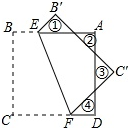
\includegraphics[width=\textwidth]{3.jpg}
	\end{column}
	\end{columns}
\end{question} \pause
\begin{answer} \pause
	\[8 * 4 = 32\]
\end{answer}
\end{frame}

\end{document}